% Figura do Cap. II: os três passos da escolha da configuração (otimização,
% ordenação pelo critério, teste só da escolhida). Criada em 05/11/2026, a pedido
% do autor, junto com a linha do tempo dos períodos. O número 312 é o total do
% Quadro da grade (Cap. II). PROPOSTA, fora do TG até o autor decidir. Compilada pelo Makefile desta pasta.
\documentclass[10pt,border=2pt]{standalone}
\usepackage[T1]{fontenc}
\usepackage[utf8]{inputenc}
\usepackage{mathptmx}
\usepackage{tikz}
\usetikzlibrary{arrows.meta,positioning,calc}
\tikzset{
  passo/.style={draw, semithick, rounded corners=2pt, fill=gray!10, align=center,
                font=\small, text width=37mm, minimum height=22mm},
  seta/.style={-{Stealth[length=2.2mm]}, semithick},
  txt/.style={font=\footnotesize, align=center},
}
\begin{document}
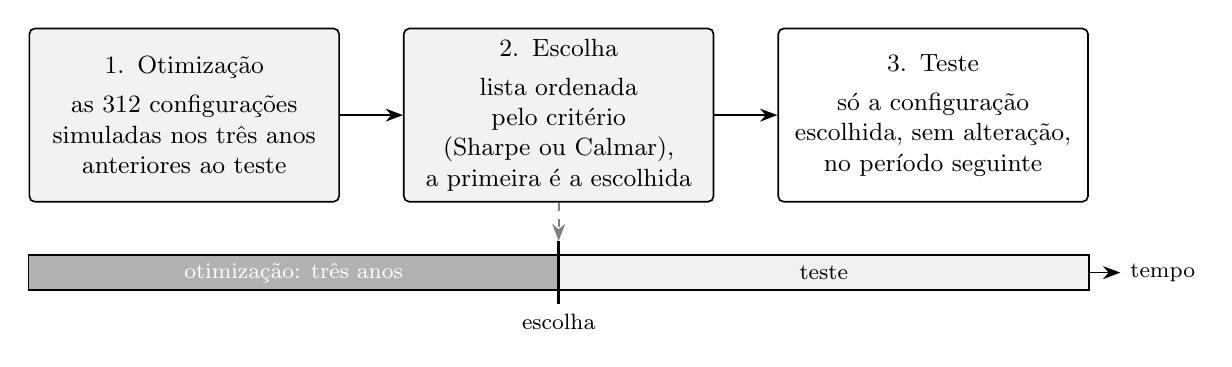
\begin{tikzpicture}
  \node[passo] (p1) at (0,0)
    {1. Otimização\\[3pt] as 312 configurações\\simuladas nos três anos\\anteriores ao teste};
  \node[passo, right=8mm of p1] (p2)
    {2. Escolha\\[3pt] lista ordenada pelo critério\\(Sharpe ou Calmar),\\a primeira é a escolhida};
  \node[passo, right=8mm of p2, fill=white] (p3)
    {3. Teste\\[3pt] só a configuração\\escolhida, sem alteração,\\no período seguinte};
  \draw[seta] (p1) -- (p2);
  \draw[seta] (p2) -- (p3);

  % linha do tempo do mesmo teste
  \coordinate (t0) at ($(p1.west)+(0,-2.0)$);
  \coordinate (t1) at (p2.south |- t0);
  \coordinate (t2) at ($(p3.east)+(0,-2.0)$);
  \filldraw[semithick, fill=gray!60] ($(t0)+(0,-0.22)$) rectangle ($(t1)+(0,0.22)$);
  \filldraw[semithick, fill=gray!12] ($(t1)+(0,-0.22)$) rectangle ($(t2)+(0,0.22)$);
  \node[txt, text=white] at ($(t0)!0.5!(t1)$) {otimização: três anos};
  \node[txt] at ($(t1)!0.5!(t2)$) {teste};
  \draw[very thick] ($(t1)+(0,-0.4)$) -- ($(t1)+(0,0.4)$);
  \node[txt, below] at ($(t1)+(0,-0.4)$) {escolha};
  \draw[seta, dashed, gray] (p2.south) -- ($(t1)+(0,0.4)$);
  \draw[seta] ($(t2)+(0,0)$) -- ++(0.4,0) node[right, txt] {tempo};
\end{tikzpicture}
\end{document}
